\section{Design}


The overarching target of \$\{PROJECT\_NAME\} is to capture Linux syscalls with low overhead. \$\{PROJECT\_NAME\} realizes syscall capturing in three steps. (1) \$\{PROJECT\_NAME\} inspect and record each syscall. (2) Next, \$\{PROJECT\_NAME\} filter these records by some arrtibutions of its caller process. (3) Finally, \$\{PROJECT\_NAME\} transfer these filtered records.

\subsection{Design Choices}

When designing \$\{PROJECT\_NAME\}, I make three design choices.

\begin{itemize}
    \item \textbf{Modify Kernel Source vs. Load Kernel Module:} Modifying Kernel source may make all procedures much more easy. However, this approach will inevitably reduce the compatibility of \$\{PROJECT\_NAME\}, especially for devices whose kernels have been modified by manufacturers. Futhermore, to modify kernel, we would also need to synchronize upstream changes. Consequently, \$\{PROJECT\_NAME\} is baesd on kernel moudle and works as a loadbale driver.
    \item \textbf{Source vs. Binary: }  I choose to do the capturing at
    the binary level instead of at the source code level. because it is quite common that source code and system calls have not corresponded (e.g., library function \texttt{malloc} do not necessarily call the \texttt{mmap}), with most programs use libraries instead of calling system calls directly. In fact, \$\{PROJECT\_NAME\} only concerns the runtime of processes, and would not perform any static analysis.
\end{itemize}

\subsection{Challenges}

To achieve its desgin goal, \$\{PROJECT\_NAME\} faces following challenges.


\subsubsection{Syscall parameters}

Considering some syscalls that allow to pass pointer and then modify its memory addressed by this pointer, it is necessary to check and record the change. For example, the prototype of syscall \texttt{getrandom} is defined as follow:\cite{getrandom2}


\centerline{\texttt{ssize\_t getrandom(void *buf, size\_t buflen, unsigned int flags);}}

It is clear that the \texttt{getrandom} will fill the buffer pointed to by its first parameter, \texttt{buf}. Therefore, \$\{PROJECT\_NAME\} needs to record the memory area changed by syscall. However, there is still a challenge that sometimes we cannot get the address at the end of syscall involked. This is due to the way the parameters are passed, determined by the architecture of CPU.

In Arm64 \cite{syscall}, both first argument(\texttt{arg1}) and return value are saved in register \texttt{r0}, which means the parameter stored in \texttt{r0} will be replaced with return value before the syscall return to user. This results in the inability to directly record the chanegs only at the end of syscall handled in kernel. I solve this challenge by adding an extra record for several syscalls.


% \subsubsection{Filter by Process}

% The capture needs filter by process due to the concurrency of the OS, i.e., interleaving with multiple processes. Thus, to distinguish the different syscall callers, \$\{PROJECT\_NAME\} has to add the caller's information for each syscall record. Accordingly, this challenge become \textit{how to get the process that issued the system call}. I address this challenge by inspecting a sepcial data structure in Linux kernel.

\subsubsection{Record Transfer}

System call records need to be stored in a buffer, while it is a very important issue when it comes to somehow get them from the buffer in real-time, with low consumption, and completely. However, the most strightforward solution, i.e., trying to keep fetching data from the buffer and save to file, causes a huge amount of overhead. I solve this challenge by enlarging buffer and reducing the frequency of acquisition.





\begin{figure}
    \centering
    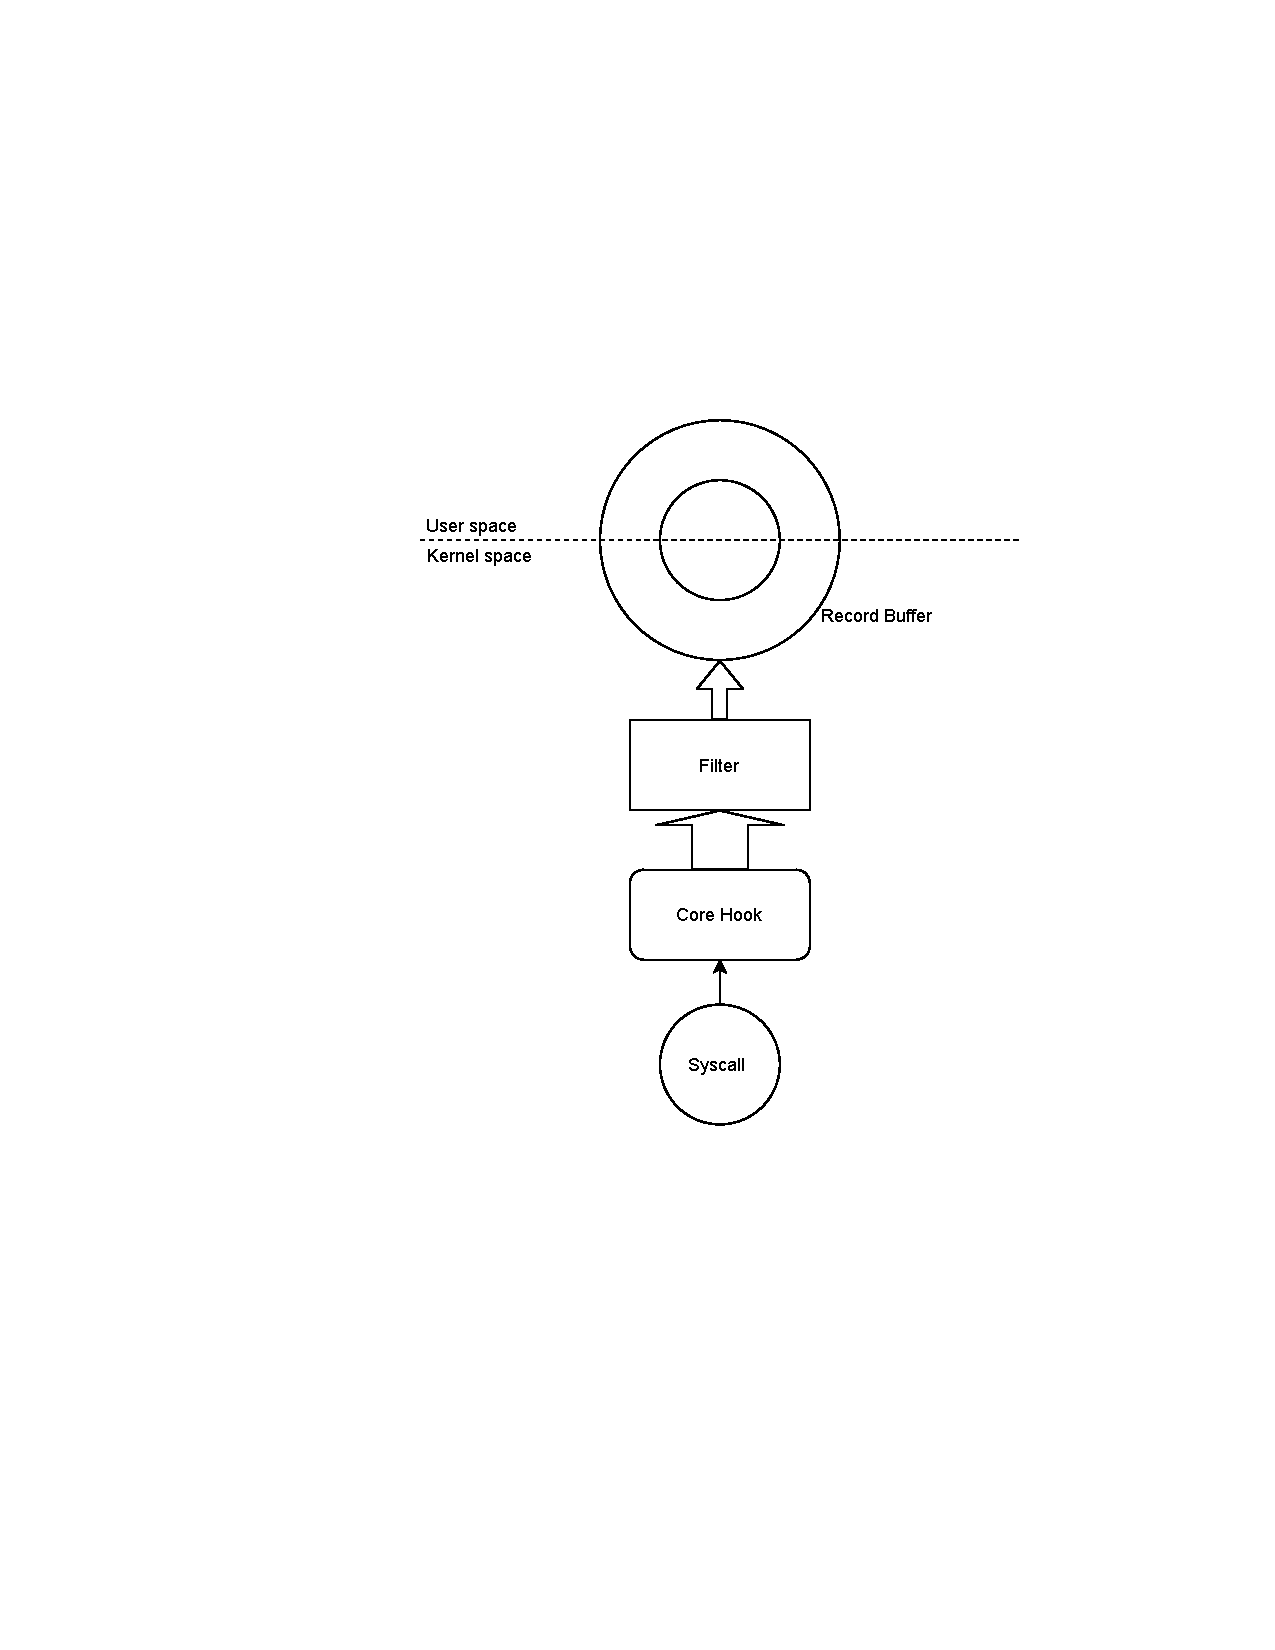
\includegraphics[width=0.5\textwidth]{figures/arch.pdf}
    \caption{The three parts of \$\{PROJECT\_NAME\}}
    \label{fig:arch}
\end{figure}



% In this section, I describe the desgin of \$\{PROJECT\_NAME\} by focusing on how it solves the above challenges

In this section, I present the desgin of \$\{PROJECT\_NAME\} by focusing on how it addresses the above three key challenges. \$\{PROJECT\_NAME\} contians three parts: \textit{core hook}, \textit{filter}, and \textit{record transfer}. 

As Figure \ref{fig:arch} shows, in the kernel space, \textit{core hook} will firslty inspect each syscall and then transfer relevant information to \textit{filter} part. Subsequently, at the \textit{filter} part, syscall records with specific features (e.g., process id or name) will be selected and finally pass to \textit{record transfer}. Meanwhile, a daemon will check the buffer periodically and dump these data form buffer to file.

\begin{figure}
    \centering
    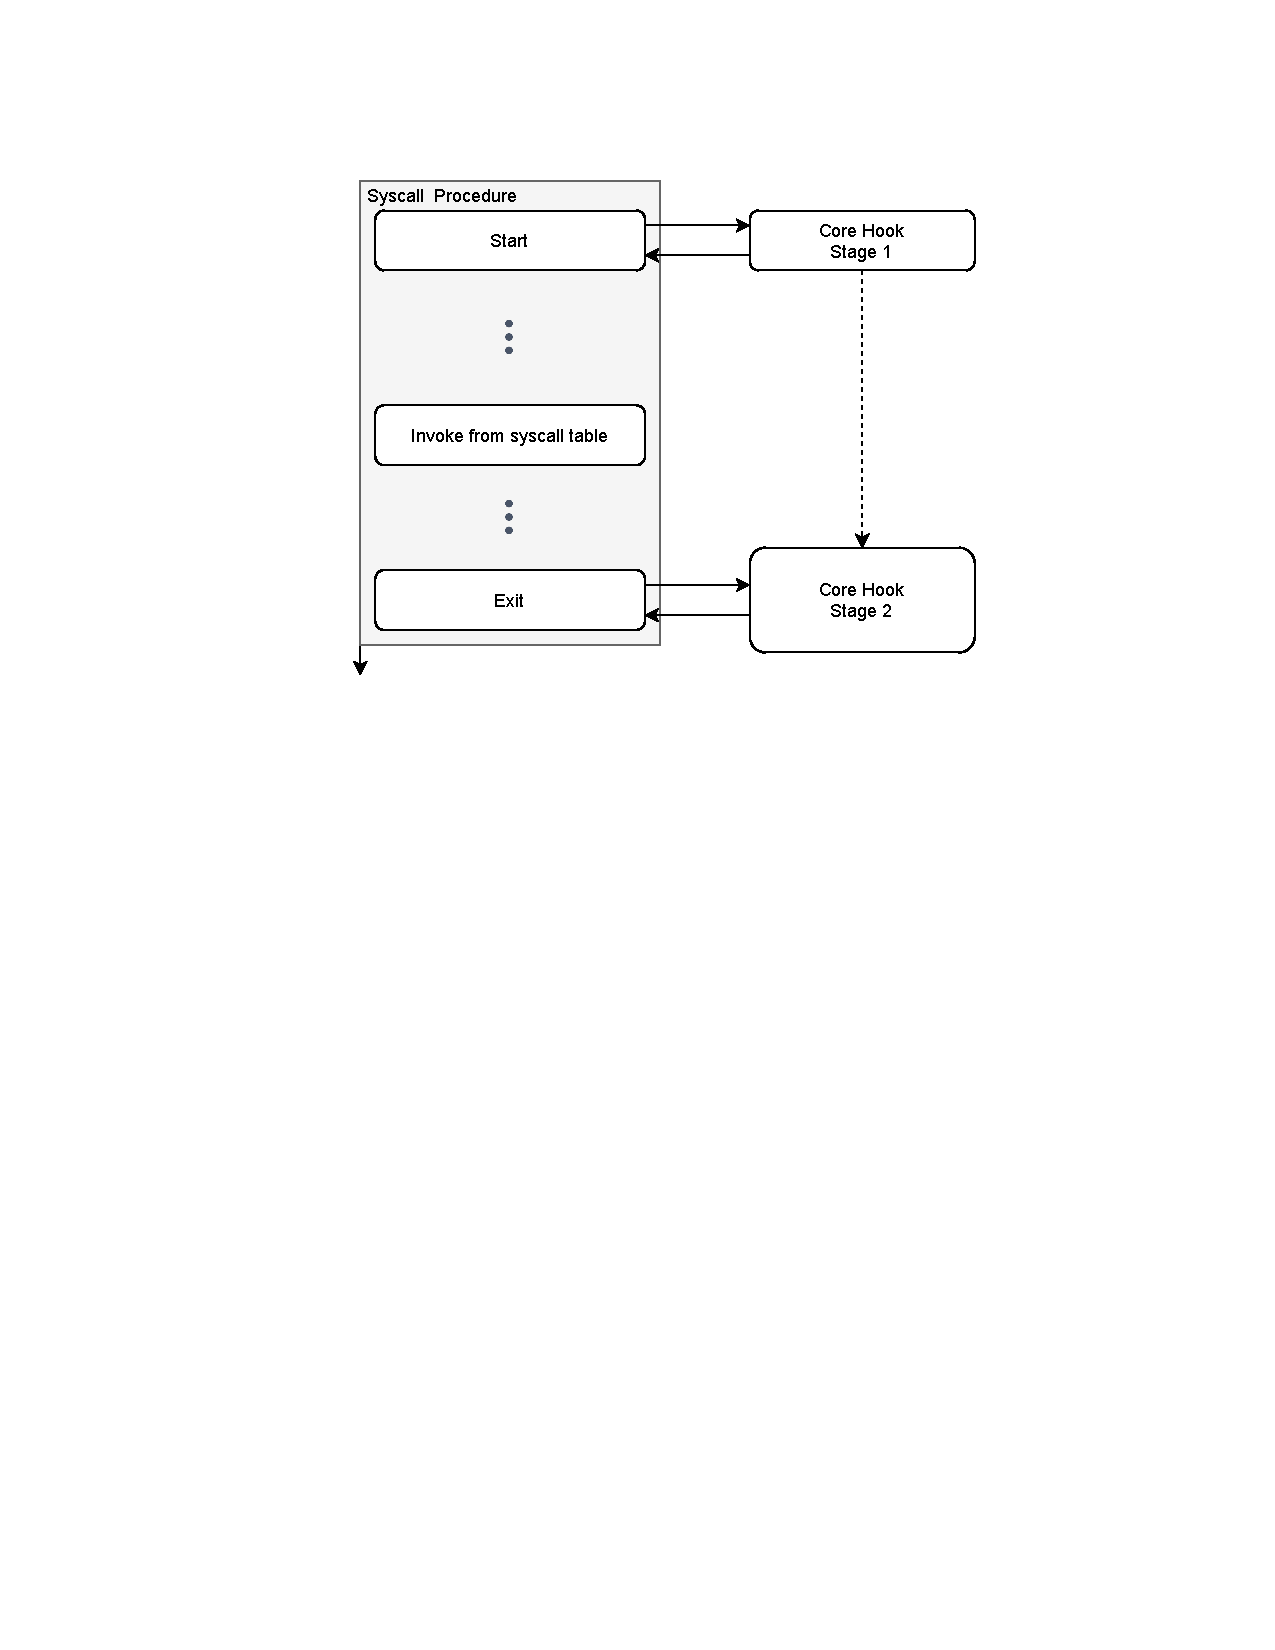
\includegraphics[width=0.5\textwidth]{figures/core-hook-desgin.pdf}
    \caption{The two tages of \textit{core hook}}
    \label{fig:core-hook-desgin}
\end{figure}


\subsection{Core Hook}

Figure \ref{fig:core-hook-desgin} shows the general workflow of \textit{core hook}. It consists of two stages of hooks, at the beginning and end of kernel handling of syscall. For the stage 1, \$\{PROJECT\_NAME\} will follow the start of syscall handlers and save the value of first parameter, if this syscall may change the memory addressed by first argument.


The second stage takes on more responsibility, including the recording of other pointer type parameters (except for the first one), and return values. Besides, this stage should also get the relevant information collected by stage 1.

There is still a problem that, due to the concurrency of the system, there may be multiple system calls being processed at the same time. Especially considering that the system calls processed in a relatively long period. So, there will be multiple system calls going to different stages of  \textit{core hook}.

This problem is solved by the observation that syscall will block the thread in user space. Therefore, we can find a one-to-one mapping from thread number to a system call event at any moment. I maintain a table to save these correspondences in second stage, and also get its first parameters from stage 1.

\subsection{Filter}

The \texttt{filter} part is a relatively simple component that requires information about the caller of the syscall from the Linux kernel. Then it will perform filter by pre-passed conditions. Last, it passes this filtered information on to the next part.

\subsection{Record Buffer}

The \textit{record buffer} is intended to act as a transit between kernel space and user space. Therefore it has two parts located in kernel space and user space respectively. One of the simplest designs is to maintain a daemon in user space constantly querying and retrieving the data stored in the buffer, and then dumping the data to a file. However, we note that this introduces a huge amount of overhead, mainly due to frequent file io. Placing a larger buffer in user space would also solve this problem, but \$\{PROJECT\_NAME\} do not want to introduce a large impact on the entire system.

Therefore, \textit{record buffer} is designed to keep fetching the buffer occupancy, and then dumps the whole buffer only after finding that the buffer occupancy has reached a threshold.